\documentclass[12pt, letterpaper,fleqn]{article}
\usepackage[utf8]{inputenc}
\usepackage{mathtools}
\usepackage{indentfirst}
\usepackage{hyperref}
\usepackage{pgfplots}
\usepackage{listings}
\usepackage{float}
\pgfplotsset{compat=1.9, width=10cm}

\usepgfplotslibrary{external}
\tikzexternalize

\DeclarePairedDelimiter\abs{\lvert}{\rvert}%

\title{Trabalho Prático 3}
\author{Hugo Silva, José Torres}
\date{novembro 2022}

\begin{document}

\maketitle

\section*{Introdução}

Visamos estudar métodos de aproximação numéricos para o cálculo de valores exatos de $f(x)$, sendo $f$ a função em questão.

Durante este trabalho iremos usufruir de \textbf{métodos de interpolação} de funções e usufruiremos também de \textbf{métodos de construção de splines} (maioritariamente cúbicas) para tais funções. 

\section*{Exercício 1}

A função a ser estudada é $f(x) = x^2 + \sin(6x)$ para $x \in \mathopen[-1,1\mathclose]$

\begin{quote}
\centering
    \begin{tikzpicture}
        \begin{axis} [xmin=-1, xmax=1, axis lines=cube, xlabel=$x$, ylabel=$y$]
            \addplot[color=red, samples=200]{x^2 + sin(deg(6*x))};
            \addlegendentry{$f(x)$}
        \end{axis}
    \end{tikzpicture}
\end{quote}

\begin{itemize}
    \item Pretende-se calcular um conjunto $n+1 = 8$ pontos, ($x_i, f_i = f(x_i)$) inicialmente. \\
    
    Para tal, calculamos atribui-se $x_0 = -1$ e $x_7 = 1$ e, consequentemente, todos os pontos intermédios irão estar divididos em parcelas aproximadamente iguais entre $x_0 e x_7$, parcelas essas que podem ser calculadas através da amplitude $h$:
    
    $$h = \frac{b-a}{n}$$
    
    %\[h = \frac{b-a}{n}\]

    Onde $\mathopen[-1,1\mathclose] = \mathopen[a,b\mathclose]$ e $n = 7$. \\
    
    Da fórmula acima indicada temos o desenvolvimento:

    $$h = \frac{1-(-1)}{7} = \frac{2}{7} \approx 0.286$$
    %\[h = \frac{1-(-1)}{7} = \frac{2}{7} \approx 0.286\]

    E finalmente temos que:
    $$x_n = x_0 + h\times n \Leftrightarrow x_n = -1 + 0.286n$$
    %\[x_n = x_0 + h\times n \Leftrightarrow x_n = -1 + 0.286n\]

    Por fim obtemos a tabela de valores:
    
    \begin{center}
        \begin{tabular} {|| c | c | c | c | c | c | c | c | c ||} \hline
            $i$ & $0$ & $1$ & $2$ & $3$ & $4$ & $5$ & $6$ & $7$\\ [0.4ex]\hline
            $x_i$ & $-1$ & $-0.714$ & $-0.428$ & $-0.142$ & $0.144$ & $0.430$ & $0.716$ & $1$ \\ [0.4ex]\hline
            $f(x_i)$ & 1.279 & 1.419 & -0.359 & -0.732 & 0.781 & 0.717 & -0.402 & 0.721 \\ [0.4ex]\hline
        \end{tabular}
    \end{center}

    \textbf{\textit{NOTA:}} Os valores de $x_i$ são arredondados devido ao facto da amplitude resultar de um valor aproximado, portanto o intervalo entre $[0.716,1]$ é mais pequeno do que o intervalo entre $[0.430, 0.716]$, porém não é algo que influencie o resultado final de forma avassaladora.

    Por ser suficiente manteve-se os intervalos representados por apenas 3 casas decimais.

    \item \textbf{\textit{Interpolação por método de Newton}} - Tendo a tabela de valores de $x_i$ disponíveis, é possível aplicar os métodos de aproximação numérica a $f(x)$.

    Comecemos pelo método de interpolação. Foi feita a escolha de usar o método de interpolação de Newton, visto que é um método mais simples para gerar o polinómio que descreve a interpolação. Em questão de geração e escrita de código, este método é um pouco mais complexo do que o método de Lagrange, visto que o método de Newton é descrito pela equação:

    \[p_n(x) = f(x_0) + (x-x_0)f[x_0,x_1] + ... + (x-x_0)...(x-x_{n-1})f[x_0, ... , x_n]\]

    O cálculo das diferenças divididas $f[x_0, ... , x_n]$ acaba por ser mais complexo algoriticamente do que a fórmula dada pelo método de Lagrange. \\
    
    Sabe-se também que uma diferença dividida de $f[x_k, ... , x_n]$ é dada pela equação:

    \[f[x_k, ... , x_n] = \frac{f[x_{k+1}, ... , x_n] - f[x_k, ..., x_{n-1}]}{x_n - x_k}\]

    Vindo de um background computacional, o grupo decidiu representar as diferenças divididas numa matrix $n\times n$.

    Suponhamos que possuímos então uma matrix $M$, onde o valor da diferença dividida numa linha $I$ e numa coluna $J$ é dada por $M[I][J]$.
    Sabe-se inicialmente que a primeira linha vai possuir os valores de $f(x_i)$ e que a partir desse ponto podemos aplicar um algoritmo que calcule o resto das diferenças. Tal algoritmo é descrito sob a forma:

    \[M[I][J] = \frac{M[I-1][J+1] - M[I-1][J]}{x_j - x_{i+j}}\]

    Seguindo o algoritmo em cima temos o código gerado:
    \begin{verbatim}
        #define LEN 7
        double m[LEN+1][LEN+1];
        double xn[LEN+1] = {-1, -0.714, -0.428, -0.142, 0.144, 0.430, 
                            0.716, 1};
    
        // f(xi) -> f[x0, ... ,xn]
        void dividedDiff() {
            // preenchimento da 1º linha com valores f(xi)
            for (int i = 0; i <= LEN; i++) {
                m[0][i] = f(xn[i]);
            }
        
            // calculo das restantes diferencas
            int limite = LEN-1; // evitar calculos impossiveis
            for (int i = 1; i <= LEN; i++) {
                for (int j = 0; j <= limite; j++) {
                    m[i][j] = (m[i-1][j+1] - m[i-1][j]) / (xn[j] - xn[i+j]);
                }
                --limite;
            }
        }
    \end{verbatim}

    Para além das diferenças divididas, existe a componente $(x-x_0)...(x-x_n)$ necessária na aplicação do método de interpolação.

    Foi denominada de função $h(x,i)$ a cada componente individual, ou seja, $h(x, 2) = (x-x_2)$:

    \begin{verbatim}
        double xn[LEN+1] = {-1, -0.714, -0.428, -0.142, 0.144, 0.430, 
                            0.716, 1};
                            
        // (x - x0)(x - x1)...(x - xn)
        double h(double x, int i) {
            return x - xn[i];
        }
    \end{verbatim}

    Basta agora aplicar o método de Newton pela definição:

    \begin{verbatim}
        // f(x0) + h(0)f[x0, x1] + ... + h(n-1)f[x0, ... , xn]
        double newton(double x) {
            // var do valor aproximado a ser calculado
            double val = 0;
        
            // var que guarda (x-x0)(x-x1)...(x-xn), etc
            double hval = 1;
        
            // aplicacao da definicao do metodo de Newton
            for (int i = 0; i <= LEN; i++) {
                val += hval*m[i][0];
                hval *= h(x, i);
            }
            
            return val;
        }
    \end{verbatim}

    \textbf{\textit{NOTA:}} Fazendo por matrix os valores de $f[x_0, ... , x_n]$ vão ficar sempre posicionados na primeira coluna ($J=0$) , sendo a razão porque apenas multiplicamos os $hval$ pelos valores $M[I][0]$ e posteriormente somamos a $val$. \\

    Prosseguiu-se ao cálculo de 200 pontos distintos através do algoritmo acima indicado, o que acabou por gerar o seguinte gráfico $p(x)$:

    \begin{quote}
        \centering
        \begin{tikzpicture}
            \begin{axis} [xmin=-1, xmax=1, axis lines=cube, xlabel=$x$, ylabel=$y$]
                \addplot[color=blue]
                table[meta=Y]
                {newtonOut.txt};
                \addlegendentry{$p(x)$}
                \addplot[color=red, samples=200]{x^2 + sin(deg(6*x))};
                \addlegendentry{$f(x)$}
            \end{axis}
        \end{tikzpicture}
    \end{quote}
    
    \item \textbf{\textit{Spline Cúbico Natural}} - Para a realização dos exercícios sobre o \textit{spline cúbico natural} foi usada a linguagem Python pelo facto de esta ter bibliotecas simples e mais fáceis de utilizar para a resolução do sistema para encontrar os valores dos multiplicadores (\textit{$M_i$}).
    
    Para encontrar os valores dos multiplicadores $M_0, M_1, ... M_n$ sabe-se que:
    
    $$\frac{h_i}{6}M_{i-1} + \frac{(h_i + h_{i+1})}{3}M_i + \frac{h_{i+1}}{6}M_{i+1} = \frac{(f_{i+1}-f_i)}{h_{i+1}} - \frac{(f_i - f_{i-1})}{h_i}, i = 1,..., n-1$$
    
    A partir desta expressão é possível criar um sistema do tipo $Ax = B$:
    
    $$
        A = \begin{bmatrix}
            1 & 0 & 0 & 0 & 0 & 0 & 0 & 0 \\[6pt]
            \frac{h}{6} & \frac{2h}{3} & \frac{h}{6} & 0 & 0 & 0 & 0 & 0 \\[6pt]
            0 & \frac{h}{6} & \frac{2h}{3} & \frac{h}{6} & 0 & 0 & 0 & 0 \\[6pt]
            0 & 0 & \frac{h}{6} & \frac{2h}{3} & \frac{h}{6} & 0 & 0 & 0 \\[6pt]
            0 & 0 & 0 & \frac{h}{6} & \frac{2h}{3} & \frac{h}{6} & 0 & 0 \\[6pt]
            0 & 0 & 0 & 0 & \frac{h}{6} & \frac{2h}{3} & \frac{h}{6} & 0 \\[6pt]
            0 & 0 & 0 & 0 & 0 & \frac{h}{6} & \frac{2h}{3} & \frac{h}{6} \\[6pt]
            0 & 0 & 0 & 0 & 0 & 0 & 0 & 1 \\
        \end{bmatrix}
        x = \begin{bmatrix}
            M_0 \\[6pt]
            M_1 \\[6pt]
            M_2 \\[6pt]
            M_3 \\[6pt]
            M_4 \\[6pt]
            M_5 \\[6pt]
            M_6 \\[6pt]
            M_7 \\[6pt]
        \end{bmatrix}
        B = \begin{bmatrix}
            0 \\[6pt] 
            -6.710 \\[6pt]
            4.916  \\[6pt]
            6.596  \\[6pt]
            -5.515 \\[6pt]
            -3.691 \\[6pt]
            7.839  \\[6pt]
            0 \\[6pt]
        \end{bmatrix}
    $$
    
    Resolvendo este sistema, usando a biblioteca \textit{numpy} e a função \textit{linalg.solve} da linguagem Python, o resultado é:
    $$
        M_i =\begin{cases}
            M_0 = 0.000   \\
            M_1 = -42.025 \\
            M_2 = 27.341  \\
            M_3 = 35.789  \\
            M_4 = -32.111 \\
            M_5 = -23.048 \\
            M_6 = 46.873  \\
            M_7 = 0.000       
        \end{cases}
    $$
    \textbf{\textit{NOTA:}} Todos os valores são arredondados a três casas decimais, já que a linguagem usada apresenta os resultados com uma precisão de 14 casas decimais.
    
    Usando os resultados do sistema acima e da expressão geral para construção de $S_i(x)$,
    $$
        S_i(x) = M_{i-1}\frac{(x_i - x)^3}{6h_i} + M_i\frac{(x-x_{i-1})^3}{6h_i}+(f_{i-1} - M_{i-1} \frac{h_i^2}{6})\frac{(x_i - x)}{h_i} + (f_i - M_i\frac{h_i^2}{6})\frac{(x-x_{i-1})}{h_i}
    $$
    obtém-se a seguinte equação do spline cúbico natural:
    \begin{equation}
        S(x) = \begin{cases}
            M_0\frac{(x_1 - x)^3}{6h} + M_1\frac{(x-x_0)^3}{6h}+(f_0 - M_0\frac{h^2}{6})\frac{(x_1 - x)}{h} + (f_1 - M_1\frac{h^2}{6}) \frac{(x-x_0)}{h}, & x_0 \leq x \leq x_1 \\
            
            M_1\frac{(x_2 - x)^3}{6h} + M_2\frac{(x-x_1)^3}{6h}+(f_1 - M_1\frac{h^2}{6})\frac{(x_2 - x)}{h} + (f_2 - M_2\frac{h^2}{6}) \frac{(x-x_1)}{h}, & x_1 \leq x \leq x_2 \\
            
            M_2\frac{(x_3 - x)^3}{6h} + M_3\frac{(x-x_2)^3}{6h}+(f_2 - M_2\frac{h^2}{6})\frac{(x_3 - x)}{h} + (f_3 - M_3\frac{h^2}{6}) \frac{(x-x_2)}{h}, & x_2 \leq x \leq x_3 \\
            
            M_3\frac{(x_4 - x)^3}{6h} + M_4\frac{(x-x_3)^3}{6h}+(f_3 - M_3\frac{h^2}{6})\frac{(x_4 - x)}{h} + (f_4 - M_4\frac{h^2}{6}) \frac{(x-x_3)}{h}, & x_3 \leq x \leq x_4 \\

            M_4\frac{(x_5 - x)^3}{6h} + M_5\frac{(x-x_4)^3}{6h}+(f_4 - M_4\frac{h^2}{6})\frac{(x_5 - x)}{h} + (f_5 - M_5\frac{h^2}{6}) \frac{(x-x_4)}{h}, & x_4 \leq x \leq x_5 \\
            
            M_5\frac{(x_6 - x)^3}{6h} + M_6\frac{(x-x_5)^3}{6h}+(f_5 - M_5\frac{h^2}{6})\frac{(x_6 - x)}{h} + (f_6 - M_6\frac{h^2}{6}) \frac{(x-x_5)}{h}, & x_5 \leq x \leq x_6 \\
            
            M_6\frac{(x_7 - x)^3}{6h} + M_7\frac{(x-x_6)^3}{6h}+(f_6 - M_6\frac{h^2}{6})\frac{(x_7 - x)}{h} + (f_7 - M_7\frac{h^2}{6}) \frac{(x-x_6)}{h}, & x_6 \leq x \leq x_7 \\
        \end{cases}    
    \end{equation}
    \textbf{\textit{NOTA:}} Optou-se por não se substituir as variáveis e constantes no sistema acima pelos respetivos valores por uma questão de formatação.
    
    O código utilizado para a construção do spline foi o seguinte:
    \begin{verbatim}
        import numpy as np
        import matplotlib.pyplot as plt 
        n = 7, h = 0.286
        # Abcissas
        xn = [-1.000, -0.714, -0.428, -0.142, 0.144, 0.430, 0.716, 1.000]
        
        # Função f(x) = x² + sin(6x)
        def f(x):
            return x**2 + (np.sin(6*x))
        # Cálculo dos valores de f(xi)
        fi = []
        for i in range(n+1):
            fi += [f(xn[i]]
        
        # Função Spline
        def spline(x):
            if xn[0] <= x <= xn[1]:
                return (M[1]*(x-xn[0])**3/(6*h))+(fi[0]*(xn[1]-x)/h) 
                        +((fi[1]-(M[1]*h**2)/6)*(x-xn[0])/h)
            (...)
        # Cálculo do sistema para encontrar os M's
        A = [ [1, 0, 0, 0, 0, 0, 0, 0],
              [h/6, 2*h/3, h/6, 0, 0, 0, 0, 0],
              [0, h/6, 2*h/3, h/6, 0, 0, 0, 0],
              [0, 0, h/6, 2*h/3, h/6, 0, 0, 0],
              [0, 0, 0, h/6, 2*h/3, h/6, 0, 0],
              [0, 0, 0, 0, h/6, 2*h/3, h/6, 0],
              [0, 0, 0, 0, 0, h/6, 2*h/3, h/6],
              [0, 0, 0, 0, 0, 0, 0, 1]                                
            ]
        B = [0]
        for i in range (1,n):
            B += [ (fi[i+1]-fi[i])/h - (fi[i]-fi[i-1])/h ]
        B += [0]
        M = np.linalg.solve(A,B)
        S = np.vectorize(spline)
        # Gráficos
        x = np.arange(start = -1, stop = 1, step = 0.001)
        y = S(x)
        ff = f(x)
        y2 = erro_spline(x)
        plt.plot(x, ff, label = 'f(x)')
        plt.plot(x, y, 'r-', label = 's(x)')
    \end{verbatim}

    O gráfico obtido com o código descrito foi o seguinte:
    \begin{figure}[H]
        \centering
        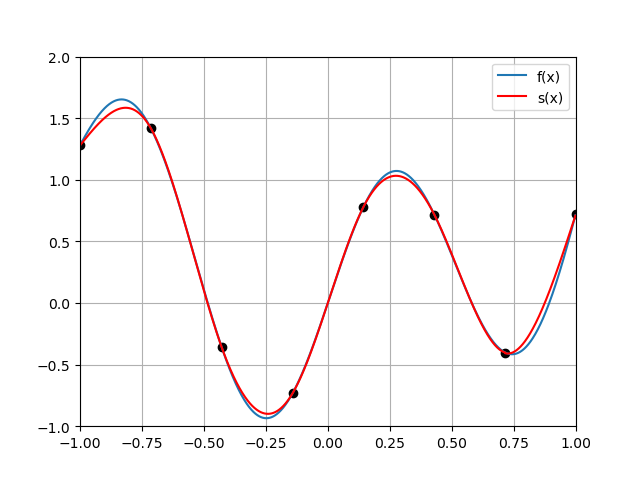
\includegraphics[width=325pt]{ex1-spline.png}
        %\caption{Spline cúbico natural do conjunto de pontos do exercício 1}
        \label{fig:spline1}
    \end{figure}
    
    \item É possível observar e comparar a capacidade de aproximação dos dois métodos comparando a $f(x)$, ou seja, observamos o comportamento que $\abs{f(x)-p(x)}$ e $\abs{f(x)-s(x)}$ tomam como gráficos:
    
    \begin{figure}[H]
        \centering
        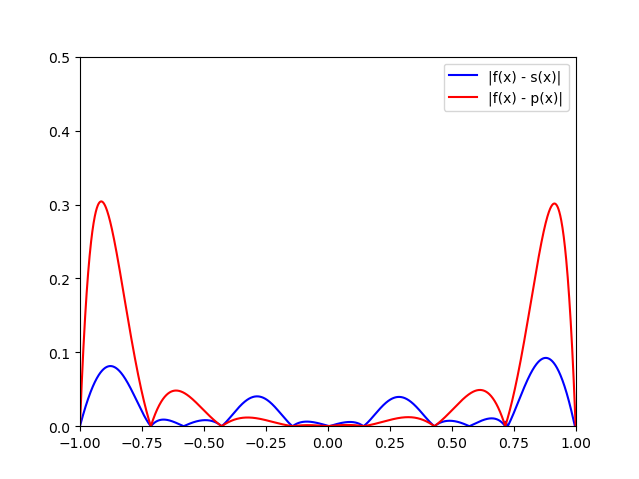
\includegraphics[width=325pt]{ex1-erros.png}
        %\caption{Caption}
        \label{fig:ex1-erros}
    \end{figure}

    Como é observável da representação gráfica acima, $s(x)$ apresenta valores mais próximos do zero, mostrando ser melhor de forma geral a aproximar os valores do que $p(x)$.

    \item Calculemos agora os erros cometidos ao calcular $f(0.1)$ e $f(0.9)$ pelos dois métodos abordados:
    \begin{itemize}
        \item \textbf{\textit{Erro (Método de Newton:)}}
            Todos os métodos de interpolação seguem o mesmo método do cálculo do erro, sendo este:
            
            $$E(x)=\frac{1}{(n+1)!}f^{n+1}(C_x)\pi_n(x)$$
            $$C_x \in \mathopen[-1,1\mathclose]$$
            $$\pi_n(x) = (x-x_0)(x-x_1)...(x-x_n)$$

            Sendo assim, tendo $n+1 = 8$ pontos, tem-se que $n = 7$:

            $$f^8(C_x) = 6^8sin(6C_x)$$

            Sabe-se que a função $sin(x)$ é contínua sendo apenas $f^8$ uma função resultante da multiplicação de constantes à função seno, logo é verificável que $f^8$ seja contínua. \\

            É pretendido fazer o majoramento do erro, logo é necessário calcular $\max(\abs{f^8(x)})$ no intervalo dado. Para tal sabe-se que entre $[1,-1]$, $\sen(x)$ passa por dois máximos locais ($-\frac{\pi}{2}$ e $\frac{\pi}{2}$), sendo assim temos que:
            $$6x = \frac{\pi}{2} \Leftrightarrow x = \frac{\pi}{12}$$

            Concluindo:
            $$\abs{f^8(\frac{\pi}{12})} = \abs{6^8\sin(\frac{\pi}{2})}$$

            Calculando as restantes componentes da equação obtém-se:
            $$E(x) = \frac{\abs{6^8\sin(\frac{\pi}{2})}}{8!}\times \pi_7(x)$$

            Basta aplicar a fórmula ao valores dados ($0.1$ e $0.9$, respetivamente):
            $$E(0.1) = 3.8\times 10^{-2}$$
            $$E(0.9) = 1.2$$
        \item \textbf{\textit{Erro (Spline Cúbico Natural:)}}
            Sabe-se que a fórmula do erro no spline cúbico natural é:
            $$E(x) \leq \frac{5}{384}Mh^4, \forall x \in [-1,1]$$
            Onde $M = max_{x\in[-1,1]}|f^{(4)}(x)|$ e $h = 0.286$. \\
            Seguindo a mesma ideia do cálculo do erro do Método de Newton, 
            $$f^{(4)} = 6^4sin(6x)$$
            $$M = |6^4sin(\frac{\pi}{2})| = 6^4 = 1296$$
            
            Assim, $E(0.1) = E(0.9) = 1.1\times10^{-1}$
    \end{itemize}
\end{itemize}

\section*{Exercício 2}

Pretende-se construir um polinómio interpolador e um spline cúbico tendo em conta os valores da seguinte tabela:

\begin{center}
    \begin{tabular} {|| c | c | c | c | c | c | c | c | c | c | c | c | c ||} \hline
        $x_i$ & $1$ & $2$ & $3$ & $4$ & $5$ & $6$ & $7$ & $8$ & $9$ & $10$ & $11$ & $12$\\ [0.4ex]\hline
        $f(x_i)$ & $8.6$ & $7.0$ & $6.4$ & $4.0$ & $2.8$ & $1.8$ & $1.8$ & $2.1$ & $3.2$ & $4.7$ & $6.2$ & $7.6$ \\ [0.4ex]\hline
    \end{tabular}
\end{center}

Visto que o método de interpolação de Newton e a construção de splines cúbicas é processo aplicado no exercício 1, anterior, usufrui-se de toda a explicação e material usado no exercício 1, obtendo-se assim o seguinte gráfico:

    %\begin{quote}
    %    \centering
    %    \begin{tikzpicture}
    %        \begin{axis} [xmin=0, xmax=13, axis lines=cube, xlabel=$x$, ylabel=$y$]
    %            \addplot[color=red]
    %            table[meta=Y]
    %            {ex2.txt};
    %            \addlegendentry{$f(x)$}
    %            %\addplot[color=green]
    %            %table[meta=Y]
    %            %{newtonOut2.txt};
    %            %\addlegendentry{$p(x)$}
    %        \end{axis}
    %    \end{tikzpicture}
    %\end{quote}
\begin{figure}[H]
    \centering
    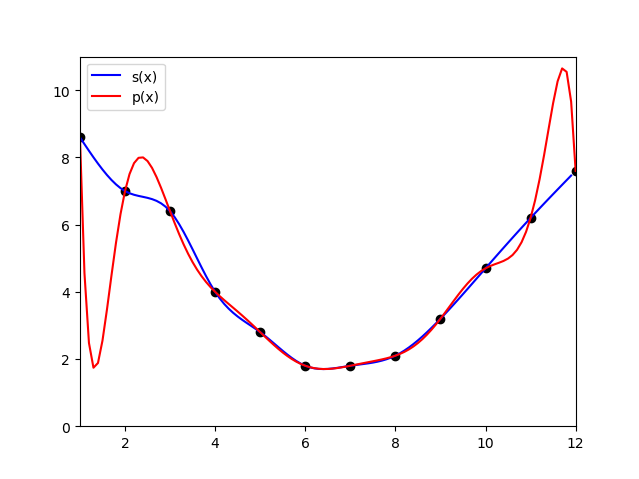
\includegraphics[width=325pt]{ex2-poly&spline.png}
    %\caption{}
    \label{fig:my_label}
\end{figure}
Com o gráfico e os valores de $f(x_i)$ é possível ver que a aproximação resultante do método do spline cúbico natural é mais precisa do que a do Método de Newton. É possível ver que nos valores iniciais, e finais, no gráfico de $p(x)$ os resultados variam enquanto que no gráfico $s(x)$ esses mesmos valores mantém-se parecidos e mais reais ao caso a ser estudado, que é a medida de evaporação da água no hemisfério sul.
\end{document}
